\documentclass[tikz]{standalone}
\usepackage{physics}
\usetikzlibrary{arrows.meta}

\begin{document}
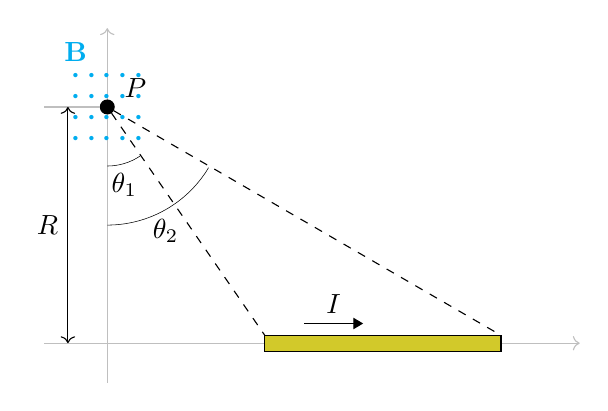
\begin{tikzpicture}
  % axis lines
  \draw[->,lightgray] (-0.8,0) -- (6,0);
  \draw[->,lightgray] (0,-0.5) -- (0,4);

  % Wire
  \draw[thin, fill=yellow!80!black, draw] (2,-0.1) rectangle (5,0.1);
  \draw[-Triangle] (2.5,0.25) --node[anchor=south]{$I$} (3.25,0.25);


  % Point
  \node[circle,draw,fill=black,inner sep=0,minimum size=5pt] (p) at (0,3){};
  \node[anchor=south west] at (p.east){$P$};

  % Dashed lines
  \draw[dashed] (p) -- (2,0.1);
  \draw[dashed] (p) -- (5,0.1);

  % Angles
  \draw[very thin] (0,3-0.75) arc [start angle=270,end angle=270+33.69,x radius=0.75cm,y radius=0.75cm] node[pos=0.5,anchor=north]{$\theta_1$};
  \draw[very thin] (0,1.5) arc [start angle=270,end angle=270+59.04,x radius=1.5cm,y radius=1.5cm]  node[pos=0.5,anchor=north]{$\theta_2$};

  % Distance R
  \draw[lightgray] (-0.8,3) -- (p);
  \draw[<->] (-0.5,0) --node[anchor=east]{$R$} (-0.5,3);

  % Magnetic field
  % a,b: x-dimensions
  % c,d: y-dimensions
  \def\a{-0.4}
  \def\b{0.4}
  \def\c{3.4}
  \def\d{2.6}
  \def\x{5}
  \def\y{4}
  \foreach \i in{1,...,\x}{
      \foreach \j in{1,...,\y}{
          \node[cyan] at ({(\b-\a)/(\x-1)*(\i-1)+\a},{(\d-\c)/(\y-1)*(\j-1)+\c}){$\vb*{\cdot}$};
        }
    }
  \node[cyan] at (-0.4,3.7){$\vb{B}$};
\end{tikzpicture}
\end{document}
